\documentclass{article}
\usepackage{graphicx}
\usepackage{geometry}
\usepackage[
    colorlinks=true,
    linkcolor=black,
    urlcolor=blue,
    citecolor=blue,
    pdfborder={0 0 0}
]{hyperref}
\usepackage{amsmath}
\usepackage{float}
\usepackage{subcaption}
\usepackage{xcolor}

\geometry{a4paper, margin=1in}

\begin{document}

\begin{titlepage}
    \centering

    {\LARGE \textbf{CSE 4208: Computer Graphics Laboratory}}\\[1 cm]

    {\Huge \textbf{Auschwitz I\\[0.3cm] Educational 3D Reconstruction}}\\[1.5cm]

    {\Large By} \\[0.5cm]
    {\Large \textbf{Raufun Ahsan}}  \\[0.3cm]
    {\Large Roll: 2007030} \\[0.8cm]

    {\Large \textbf{Submitted to}} \\[0.5cm]

    \begin{minipage}[t]{0.48\textwidth}
        \raggedright
        {\large \textbf{Dr. Sk. Md. Masudul Ahsan}} \\
        Professor \\
        Department of Computer Science and Engineering \\
        Khulna University of Engineering \& Technology
    \end{minipage}%
    \hfill
    \begin{minipage}[t]{0.48\textwidth}
        \raggedright
        {\large \textbf{Md Tajmilur Rahman}} \\
        Lecturer \\
        Department of Computer Science and Engineering \\
        Khulna University of Engineering \& Technology
    \end{minipage}

    \vfill

    
\includegraphics[width=0.3\textwidth]{assets/kuet.png} \\[1cm]

    {\Large \textbf{Department of Computer Science and Engineering}} \\[0.2cm]
    {\Large \textbf{Khulna University of Engineering \& Technology}} \\[0.2cm]
    {\Large \textbf{Khulna 9203, Bangladesh}} \\

\end{titlepage}

\tableofcontents
\newpage
\listoffigures
\newpage

\section{Introduction}
This project is a real-time OpenGL 3.3 reconstruction of Auschwitz I, implemented in C++17 with a modular scene architecture. The current implementation is centered around a zone-based world model, multi-pass rendering, and runtime interaction systems.

The implementation focuses on:
\begin{itemize}
    \item clean separation of world sectors into independent zone modules,
    \item reusable primitive-driven modeling (cube, cylinder, sphere, plane, pyramid),
    \item dynamic lighting with bounded light budgets,
    \item procedural geometry for trees and curved structures,
    \item interactive controls for scene behavior, visualization mode, and material/lighting toggles.
\end{itemize}

\section{System Architecture}
\subsection{Core Orchestration}
The entry point in \texttt{src/main.cpp} initializes GLFW/GLAD, shaders, input callbacks, and the frame loop. The central orchestrator \texttt{src/Scene.h} owns all subsystems and zones, controls texture loading/fallback, and executes the full render pipeline.

\subsection{Zone-based World Composition}
The world is built from dedicated modules under \texttt{src/zones/}, including:
\begin{itemize}
    \item \texttt{GroundZone}, \texttt{BarrackGrid}, \texttt{BarrackInteriors},
    \item \texttt{EntranceGate}, \texttt{FenceSystem}, \texttt{GuardTowers}, \texttt{StreetLamps},
    \item \texttt{Block11Zone}, \texttt{CrematoryZone}, \texttt{AdminZone},
    \item \texttt{TrainSystem} (line + locomotive + five bogeys),
    \item \texttt{SoldiersCourtyard} (formation grid + parade animation).
\end{itemize}

\subsection{World Scale Notes}
Barrack placement currently renders 24 barracks in a 4x6 grid with fixed row/column centers and consistent spacing. The entrance gate is positioned on the eastern side, while the train line is parallel to the entrance fence and outside the perimeter.

\section{Rendering Pipeline}
The frame is rendered in seven passes:
\begin{enumerate}
    \item Skybox,
    \item Stars,
    \item Opaque geometry (Phong),
    \item Celestial/unlit emissive bodies,
    \item Alpha/transparency pass,
    \item Particle pass,
    \item HUD pass.
\end{enumerate}

This organization keeps opaque and transparent content separate, supports atmosphere effects, and allows HUD rendering after scene compositing.

\subsection{4-Point View Mode}
A dedicated viewport mode splits the screen into four equal quadrants and renders:
\begin{itemize}
    \item X-axis perspective,
    \item Y-axis perspective,
    \item Z-axis perspective,
    \item isometric perspective.
\end{itemize}
This mode is toggleable at runtime and reuses the same scene rendering path per quadrant.

\begin{figure}[H]
    \centering
    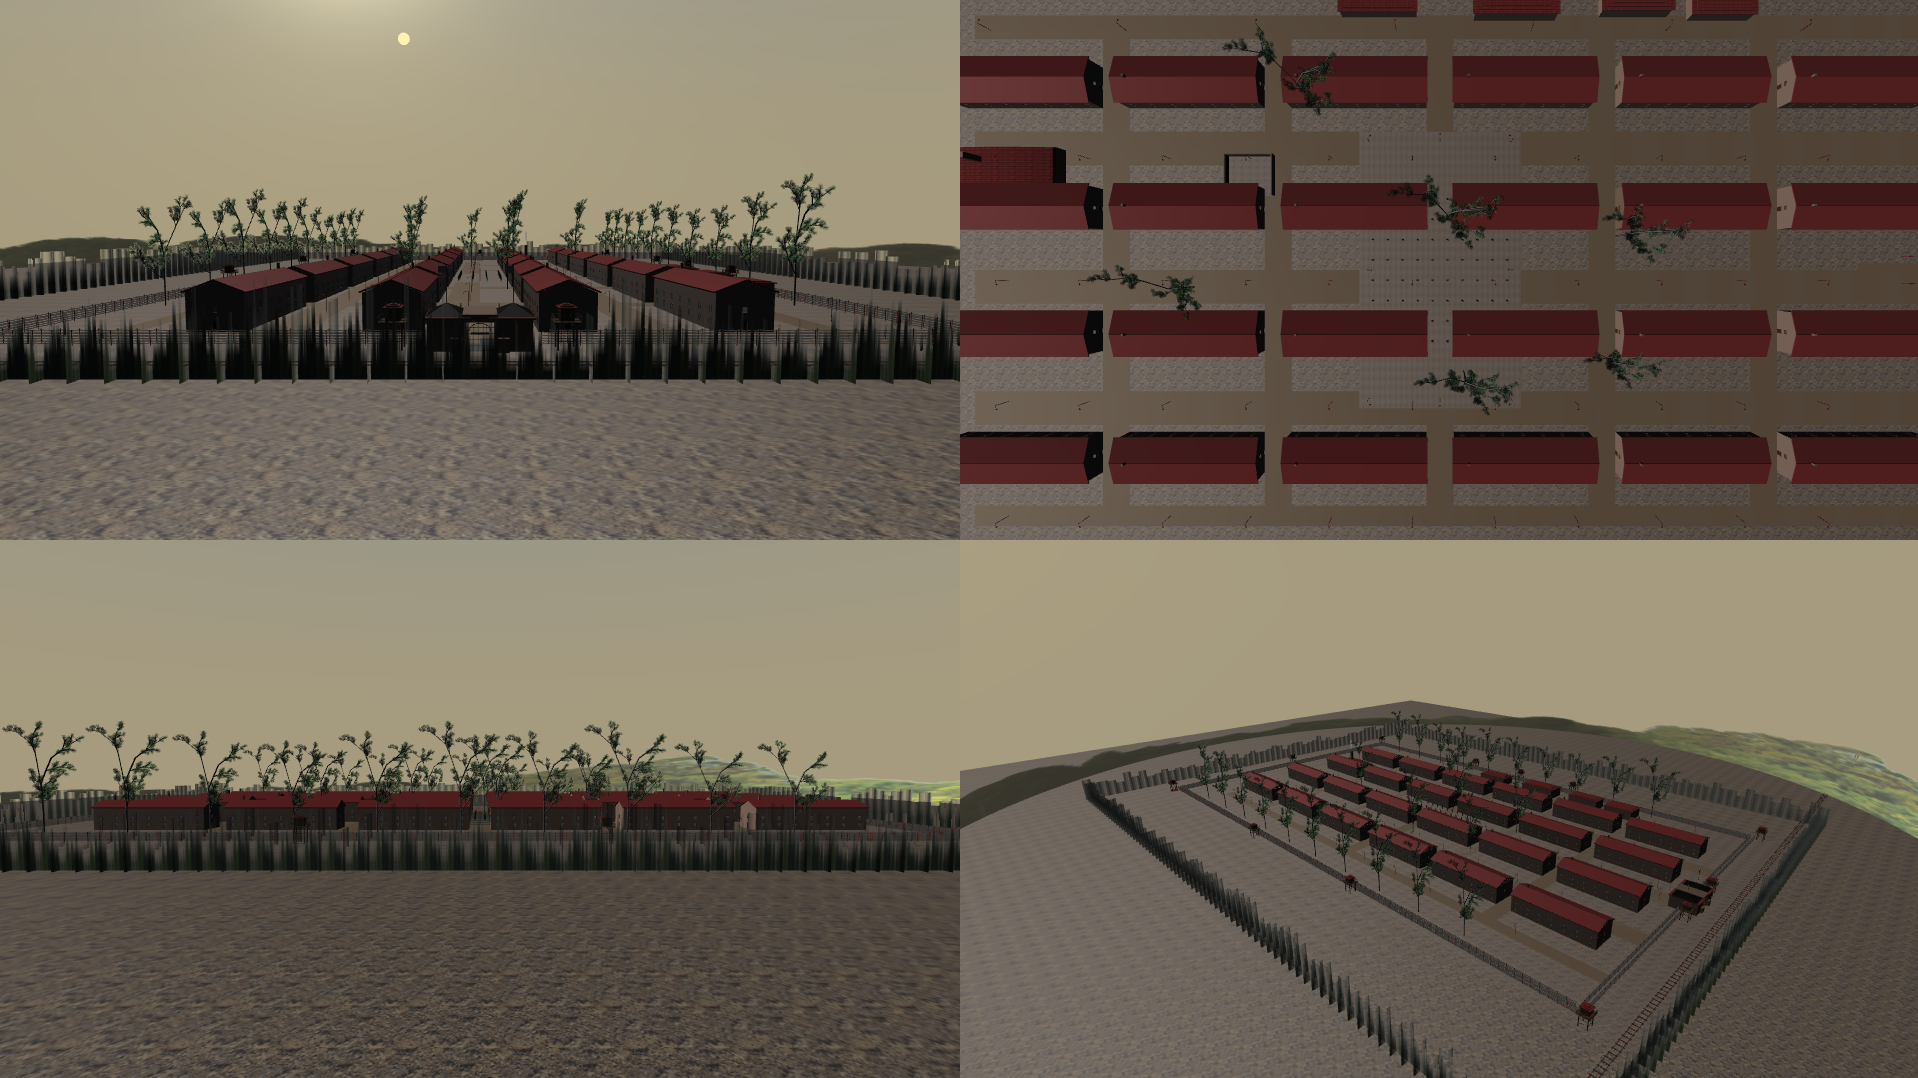
\includegraphics[width=0.9\textwidth]{assets/screenshots/camp_day.png}
    \caption{4-point view mode (day) showing X, Y, Z, and isometric perspectives.}
\end{figure}

\section{Geometry and Modeling Details}
\subsection{Primitive-based Construction}
Most structures are assembled from shared primitive meshes, with transformation-based composition for walls, roofs, poles, rails, furniture, and character parts.

Primitive roles in this project:
\begin{itemize}
    \item \textbf{Cube}: main building blocks (walls, floors, roofs, frames, furniture, soldier body parts).
    \item \textbf{Cylinder}: poles, columns, lamp posts, tower legs, and circular structural members.
    \item \textbf{Sphere}: moon/sun bodies, lamp bulbs, and rounded character features.
    \item \textbf{Plane}: large ground and road surfaces, courtyard pads, and horizon extensions.
    \item \textbf{Pyramid}: decorative roof caps and entrance-gate details.
\end{itemize}

\subsection{Curved Surfaces}
Curved elements use Bezier and ruled-surface generation.

Cubic Bezier centerline:
\begin{equation}
\mathbf{B}(t) = (1-t)^3\mathbf{P}_0 + 3(1-t)^2t\mathbf{P}_1 + 3(1-t)t^2\mathbf{P}_2 + t^3\mathbf{P}_3,
\end{equation}
\begin{equation}
\mathbf{T}(t) = \frac{d\mathbf{B}(t)/dt}{\|d\mathbf{B}(t)/dt\|}.
\end{equation}

Tube sweep around the curve frame:
\begin{equation}
\mathbf{S}(t,\theta) = \mathbf{B}(t) + r\big(\cos\theta\,\mathbf{N}(t) + \sin\theta\,\mathbf{B}_f(t)\big).
\end{equation}

Ruled surface interpolation between two boundary curves:
\begin{equation}
\mathbf{R}(u,v) = (1-v)\mathbf{C}_1(u) + v\mathbf{C}_2(u).
\end{equation}

These are used for features such as curved lamp arms, gate arch components, train boiler shape, and crematory roof profiles.

\subsection{Procedural Objects}
Besides curved surfaces, the scene uses procedural updates for trees, stars, and particles:

\textbf{L-system branch scaling (tree recursion):}
\begin{equation}
L_{k+1} = \alpha L_k, \quad r_{k+1} = \beta r_k, \quad 0<\alpha,\beta<1.
\end{equation}

\textbf{Upper-hemisphere star sampling:}
\begin{equation}
\mathbf{p}(\theta,\phi)=R\begin{bmatrix}
\cos\phi\cos\theta \\
\sin\phi \\
\cos\phi\sin\theta
\end{bmatrix},
\quad \theta\in[0,2\pi],\;\phi\in\left[0,\tfrac{0.45\pi}{ }\right].
\end{equation}

\textbf{Particle position update (snow/smoke style integration):}
\begin{equation}
\mathbf{x}_{t+\Delta t}=\mathbf{x}_t+\mathbf{v}_t\,\Delta t.
\end{equation}

\subsection{Flyweight-based Optimization}
The project uses a flyweight-style mesh container (\texttt{MeshFlyweight}) for generated meshes. Shared VAO/VBO/EBO data is created once and reused for repeated draws with different transforms/material state. This reduces duplicate geometry allocation for repeated curved assets.

\section{Lighting and Time System}
\subsection{Lighting Budget}
The Phong shader path supports:
\begin{itemize}
    \item 2 directional lights (sun + moon),
    \item up to 32 point lights,
    \item up to 36 spot lights.
\end{itemize}

\subsection{Dynamic Behavior}
The day-night cycle updates sun/moon direction and intensity continuously. Night behavior includes lamp activation, stars, and moving tower searchlights.

\subsection{Bounded Light Upload}
To keep active light counts stable:
\begin{itemize}
    \item interior point lights are selected by distance,
    \item lamp spotlights are sorted by camera distance and capped,
    \item one spotlight slot is reserved for the train headlight.
\end{itemize}

\subsection{Universal Runtime Material/Lighting Toggles}
Global keyboard controls allow toggling ambient, diffuse, specular, emissive terms and all texture sampling. This supports direct visual inspection of material and light contributions.

\section{Feature Implementations}
\subsection{Train System}
The train subsystem introduces an external rail line (two metal rails + wooden sleepers) and an animated train with one engine and five bogeys. Motion state is scripted as:
\begin{enumerate}
    \item approach from outside horizon,
    \item stop near gate,
    \item depart past horizon.
\end{enumerate}
A front spotlight is integrated into the global spotlight upload path.

\begin{figure}[H]
    \centering
    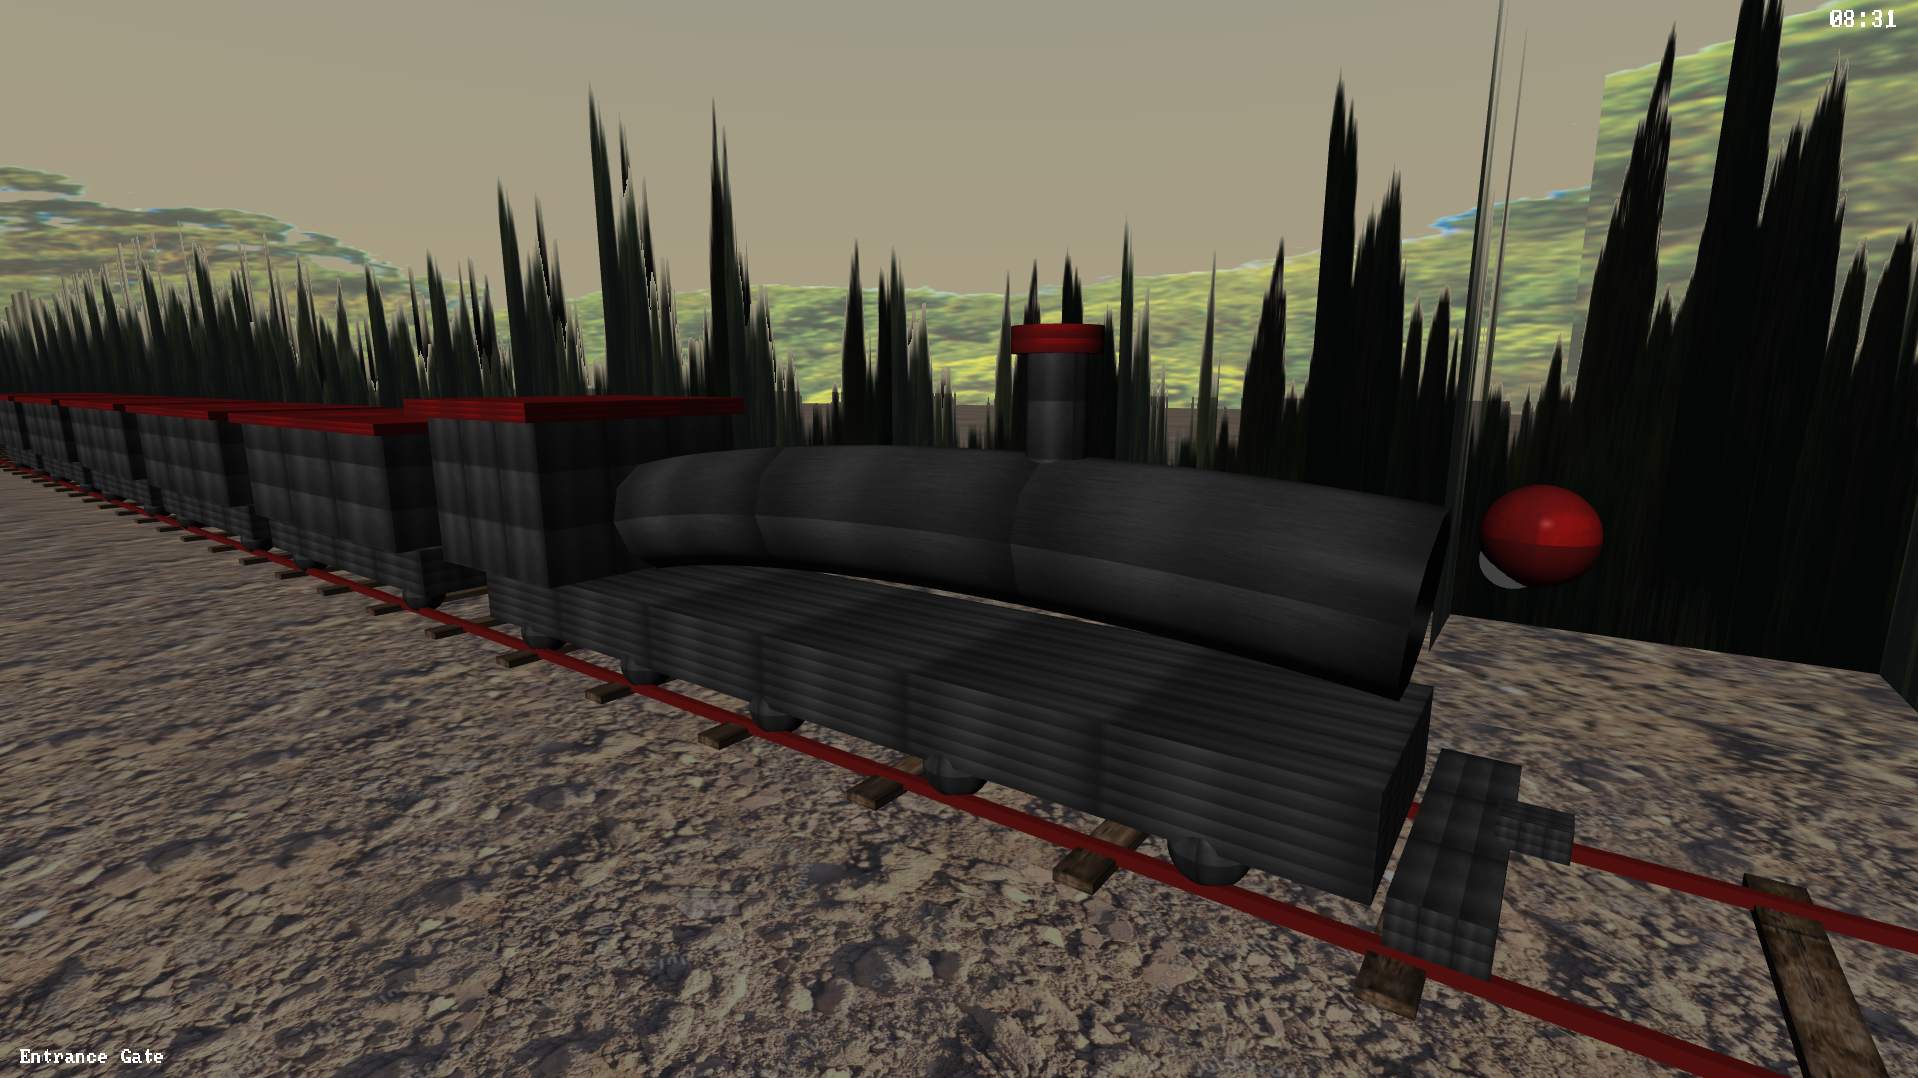
\includegraphics[width=0.8\textwidth]{assets/screenshots/train.png}
    \caption{Train system placed outside the entrance-side fence.}
\end{figure}

\subsection{Soldiers Courtyard}
A central courtyard includes a grid of primitive human figures (body, head, arms, hands, legs, feet, back-mounted rifle). Parade mode animates arm swing and leg gait while maintaining planted feet behavior.

\begin{figure}[H]
    \centering
    \begin{subfigure}{0.48\textwidth}
        \centering
        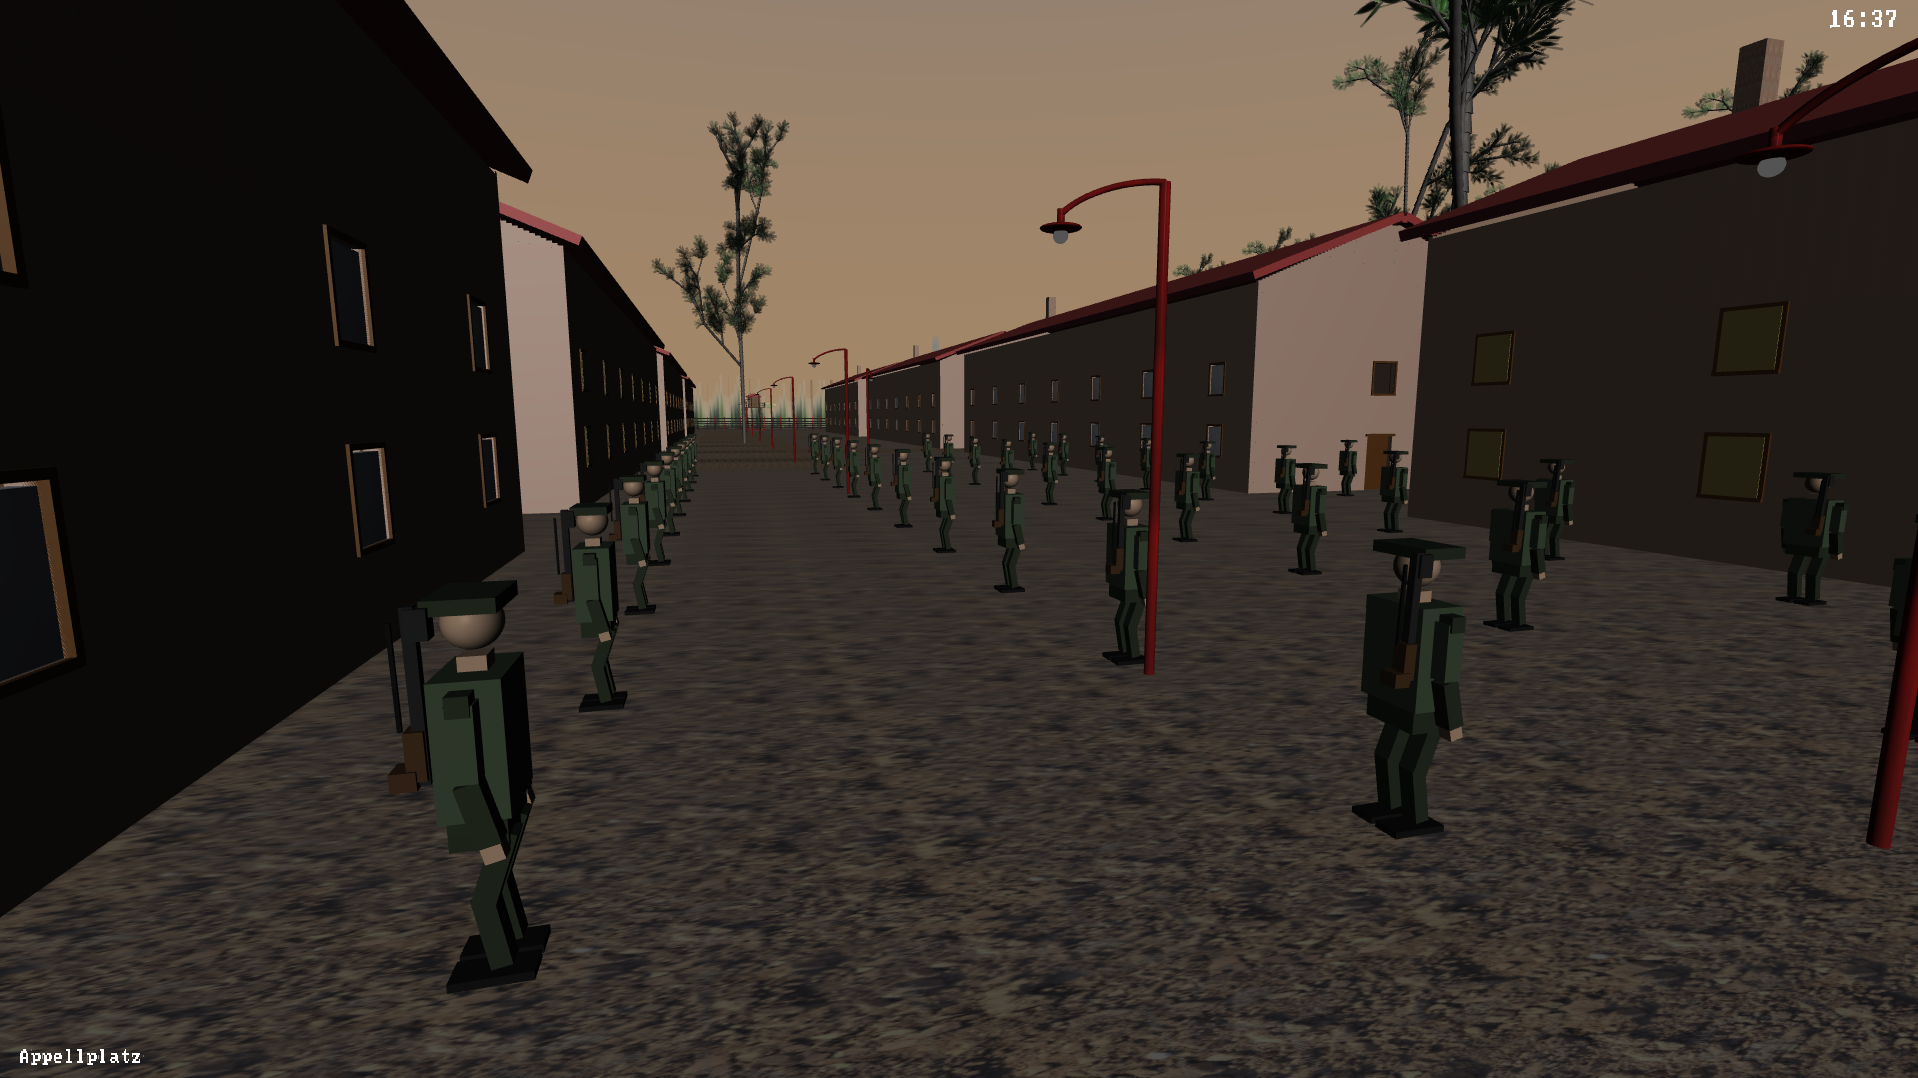
\includegraphics[width=\textwidth]{assets/screenshots/army_parade.png}
        \caption{Courtyard formation}
    \end{subfigure}
    \hfill
    \begin{subfigure}{0.48\textwidth}
        \centering
        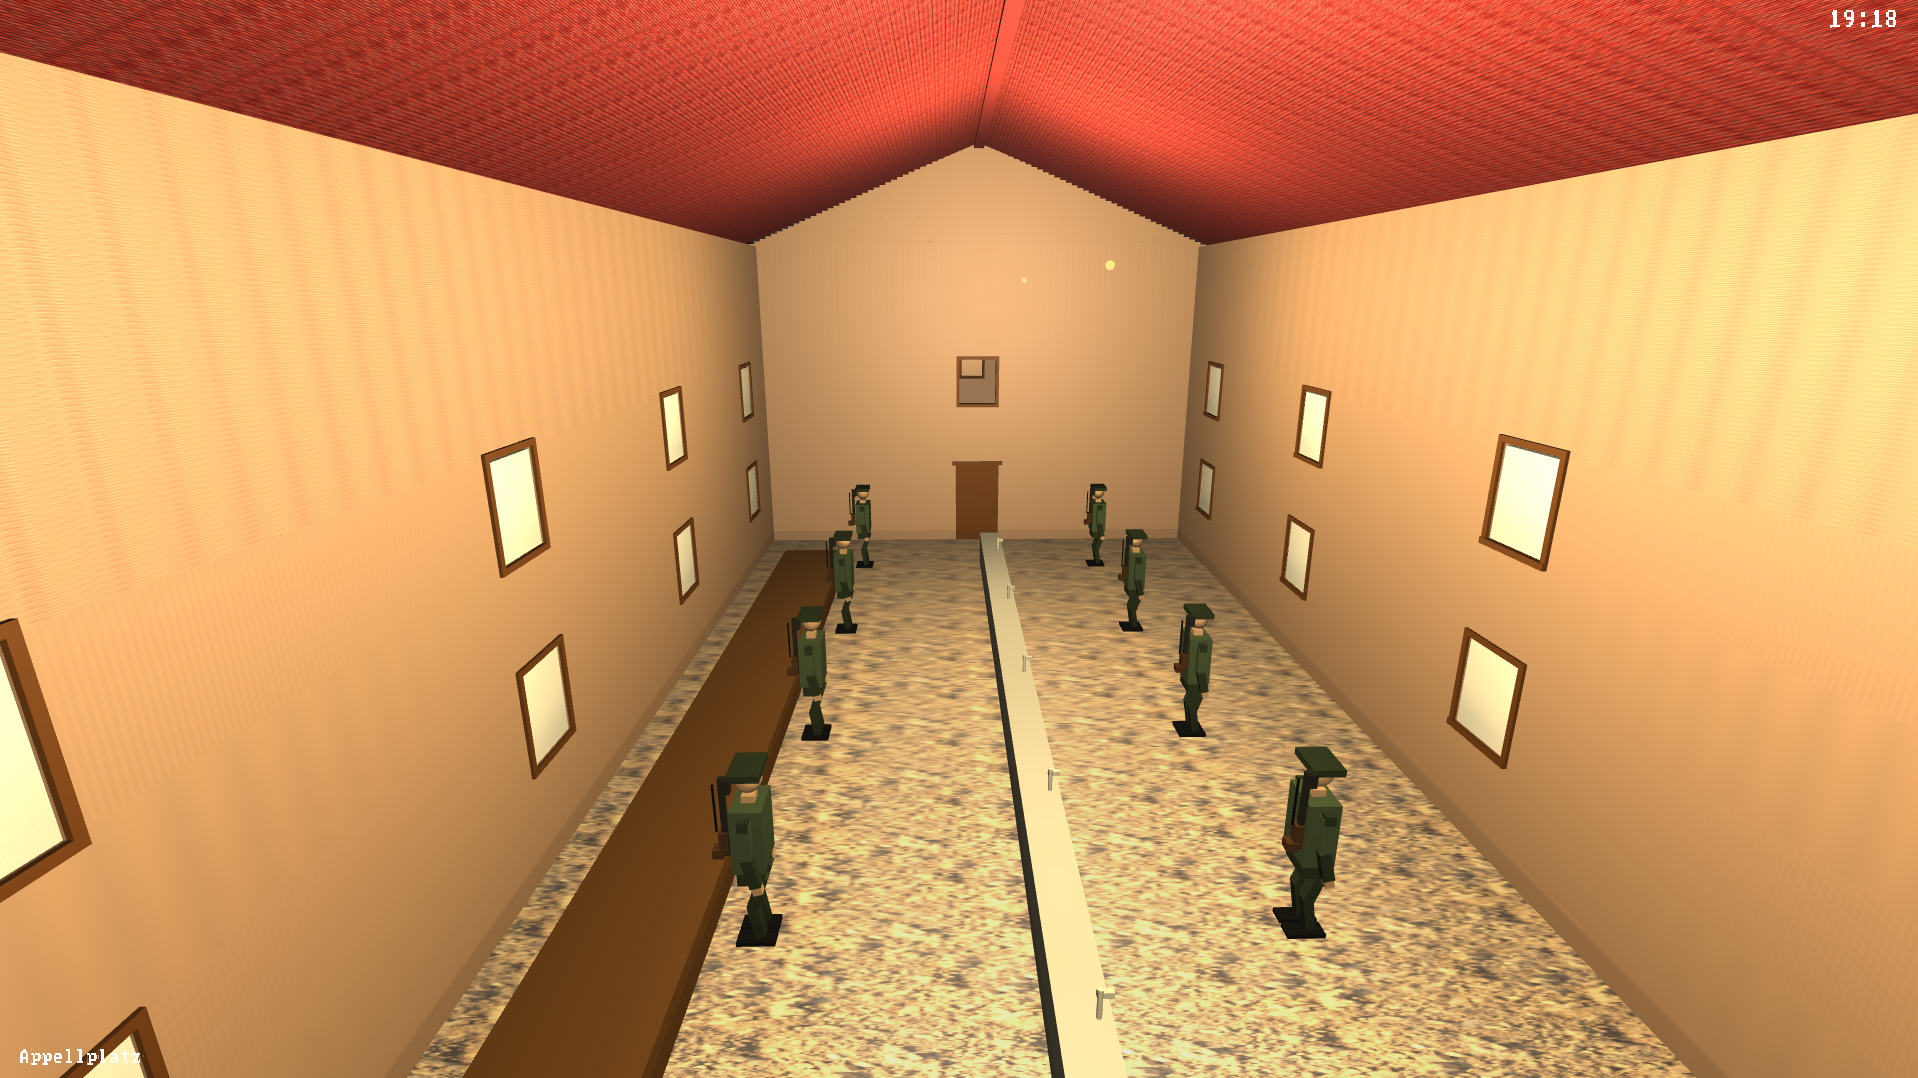
\includegraphics[width=\textwidth]{assets/screenshots/interior_army.png}
        \caption{Formation in enclosed space}
    \end{subfigure}
    \caption{Primitive soldier modeling and parade placement.}
\end{figure}

\subsection{Interiors and Distinct Zones}
The project includes dedicated zone logic for barracks, gate, administrative area, crematory area, and special block interiors (including jail-style interior layout for Block 11).

\begin{figure}[H]
    \centering
    \begin{subfigure}{0.48\textwidth}
        \centering
        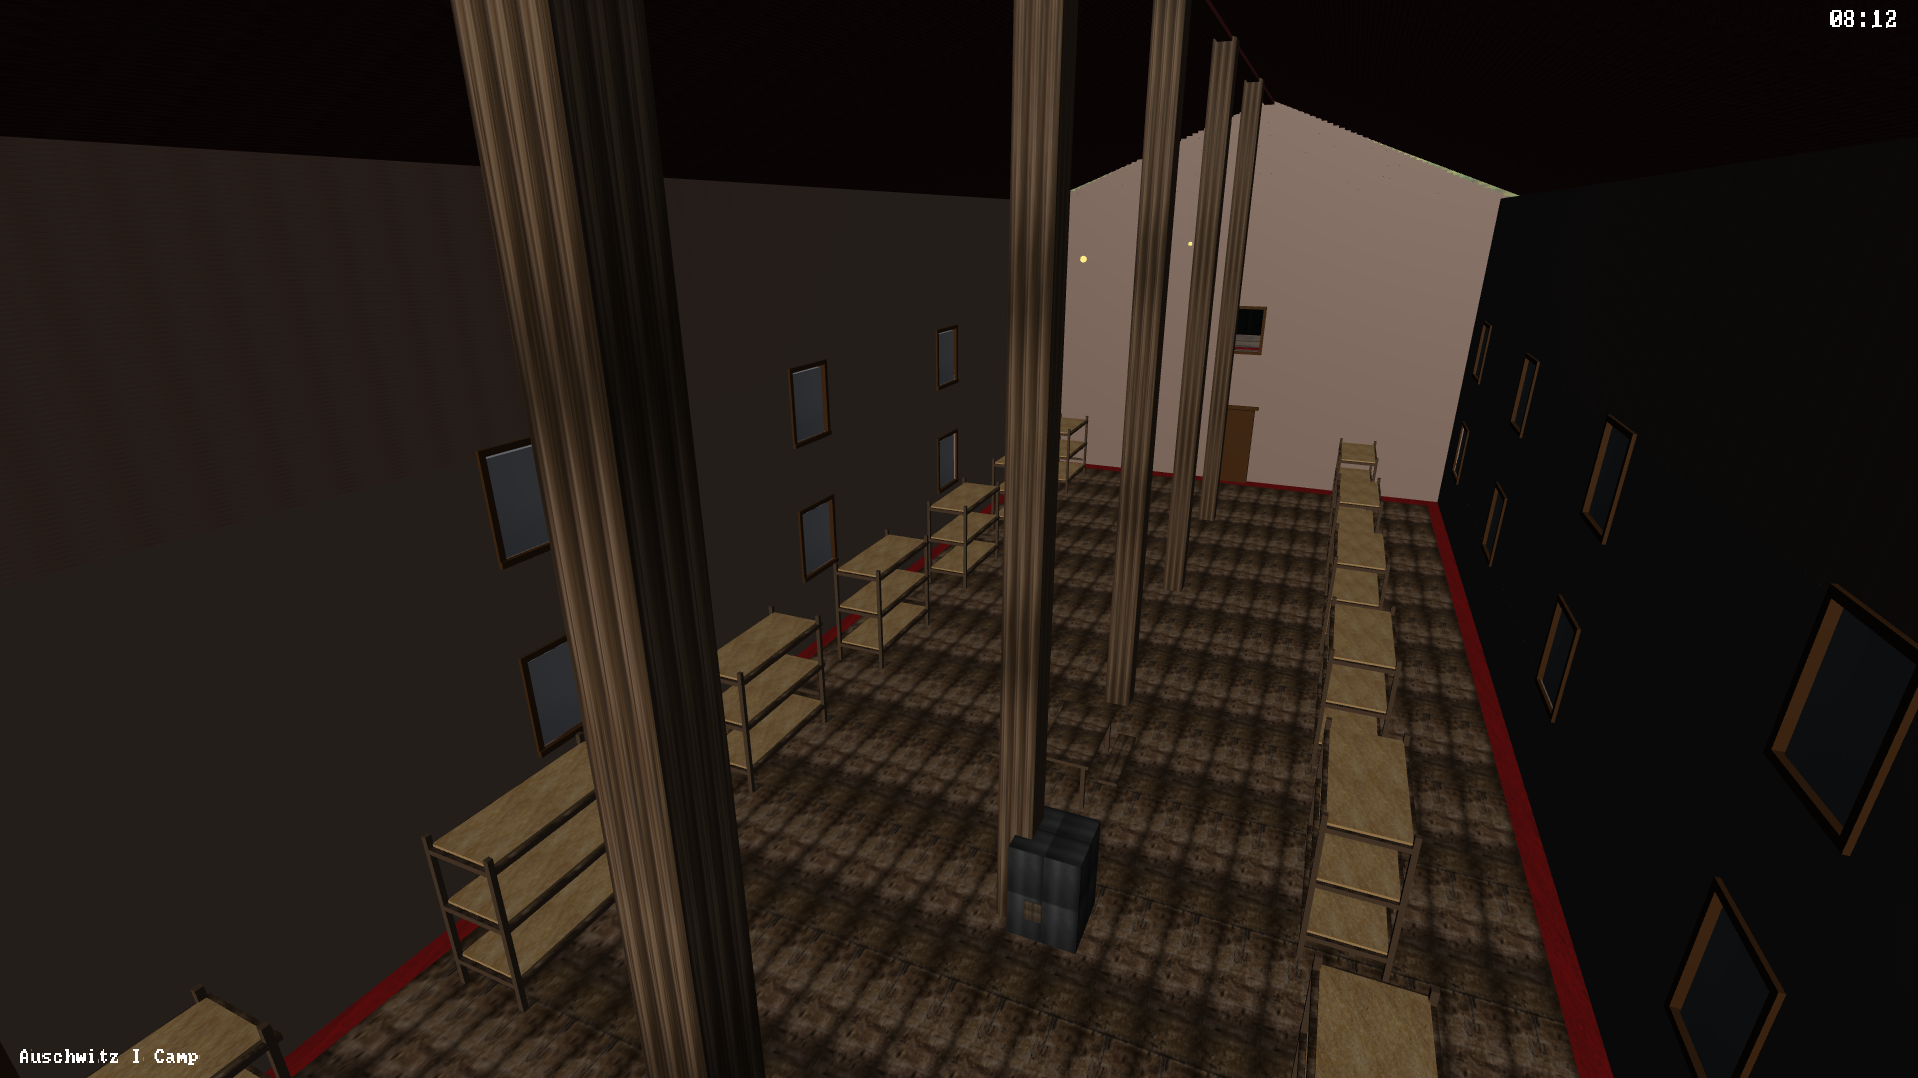
\includegraphics[width=\textwidth]{assets/screenshots/interior_house.png}
        \caption{House-style interior}
    \end{subfigure}
    \hfill
    \begin{subfigure}{0.48\textwidth}
        \centering
        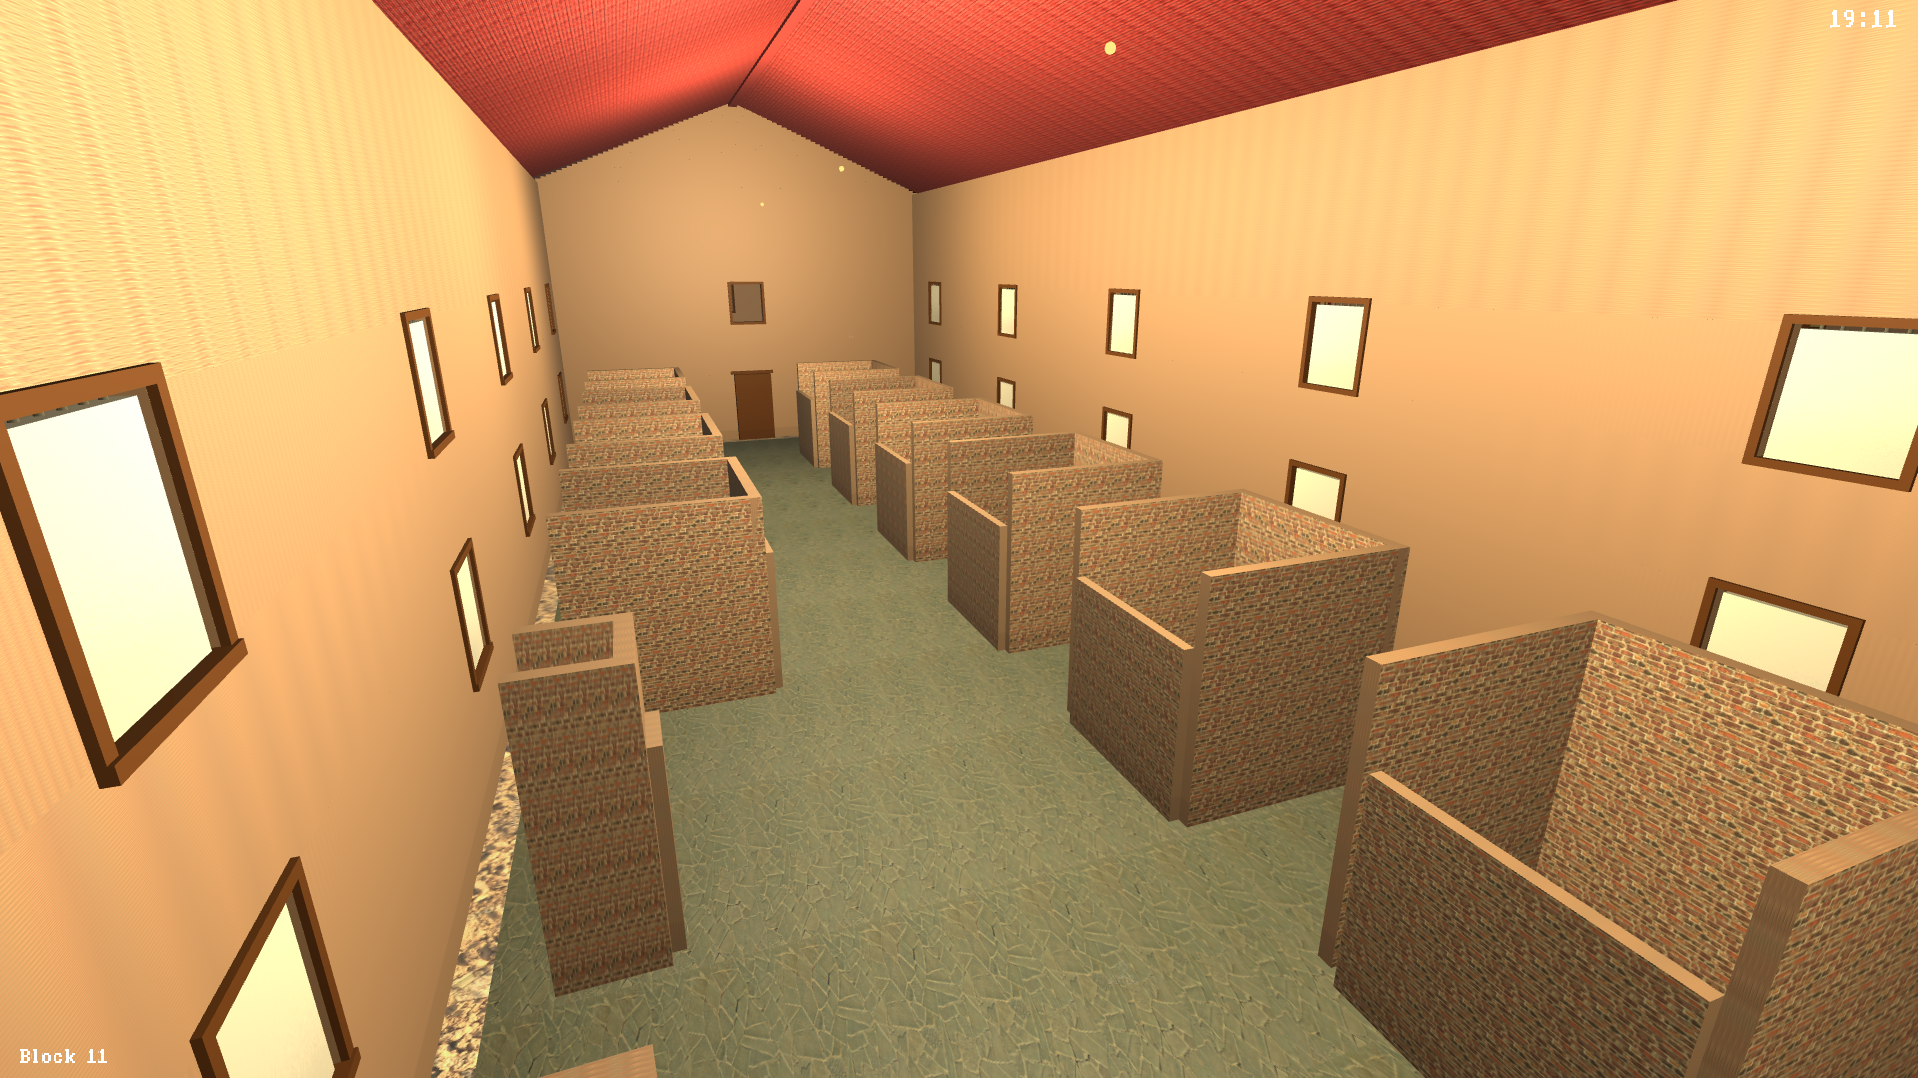
\includegraphics[width=\textwidth]{assets/screenshots/interior_jail.png}
        \caption{Jail-style interior}
    \end{subfigure}
    \caption{Interior variants used across zone implementations.}
\end{figure}

\section{Texture Pipeline and Samples}
\subsection{Texture Handling}
Textures are loaded from relative paths and used with repeat/clamp behavior depending on target surface. If a texture is unavailable, fallback solid textures are generated to keep rendering stable.

\subsection{Texture Sample Sheet}
Figure \ref{fig:texture-samples} contains all currently provided texture samples from \texttt{assets/texture\_samples/}.

\begin{figure}[H]
    \centering
    \begin{subfigure}{0.18\textwidth}\centering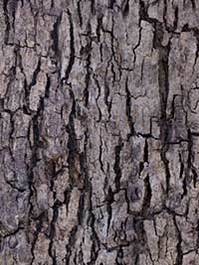
\includegraphics[width=0.9\textwidth]{assets/texture_samples/bark.png}\caption*{bark}\end{subfigure}
    \begin{subfigure}{0.18\textwidth}\centering
\includegraphics[width=0.9\textwidth]{assets/texture_samples/black_metal.png}\caption*{black\_metal}\end{subfigure}
    \begin{subfigure}{0.18\textwidth}\centering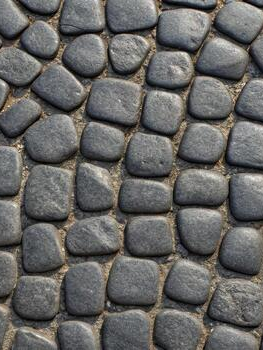
\includegraphics[width=0.9\textwidth]{assets/texture_samples/cobblestone.png}\caption*{cobblestone}\end{subfigure}
    \begin{subfigure}{0.18\textwidth}\centering
\includegraphics[width=0.9\textwidth]{assets/texture_samples/concrete.png}\caption*{concrete}\end{subfigure}

    \vspace{0.3cm}

    \begin{subfigure}{0.18\textwidth}\centering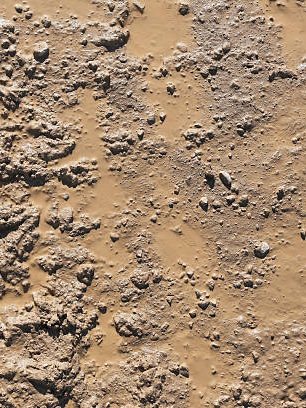
\includegraphics[width=0.9\textwidth]{assets/texture_samples/dirt_road.png}\caption*{dirt\_road}\end{subfigure}
    \begin{subfigure}{0.18\textwidth}\centering
\includegraphics[width=0.9\textwidth]{assets/texture_samples/glass_alpha.png}\caption*{glass\_alpha}\end{subfigure}
    \begin{subfigure}{0.18\textwidth}\centering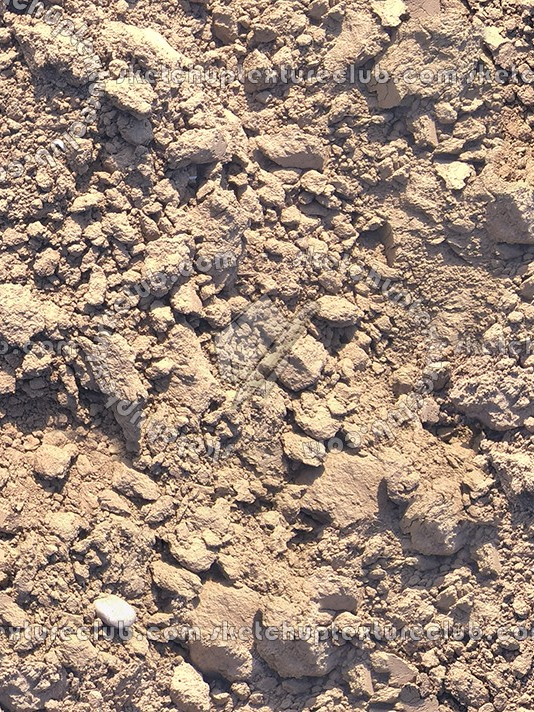
\includegraphics[width=0.9\textwidth]{assets/texture_samples/gravel.png}\caption*{gravel}\end{subfigure}
    \begin{subfigure}{0.18\textwidth}\centering
\includegraphics[width=0.9\textwidth]{assets/texture_samples/leaf_alpha.png}\caption*{leaf\_alpha}\end{subfigure}

    \vspace{0.3cm}

    \begin{subfigure}{0.18\textwidth}\centering
\includegraphics[width=0.9\textwidth]{assets/texture_samples/metal_grey.png}\caption*{metal\_grey}\end{subfigure}
    \begin{subfigure}{0.18\textwidth}\centering
\includegraphics[width=0.9\textwidth]{assets/texture_samples/metal_iron.png}\caption*{metal\_iron}\end{subfigure}
    \begin{subfigure}{0.18\textwidth}\centering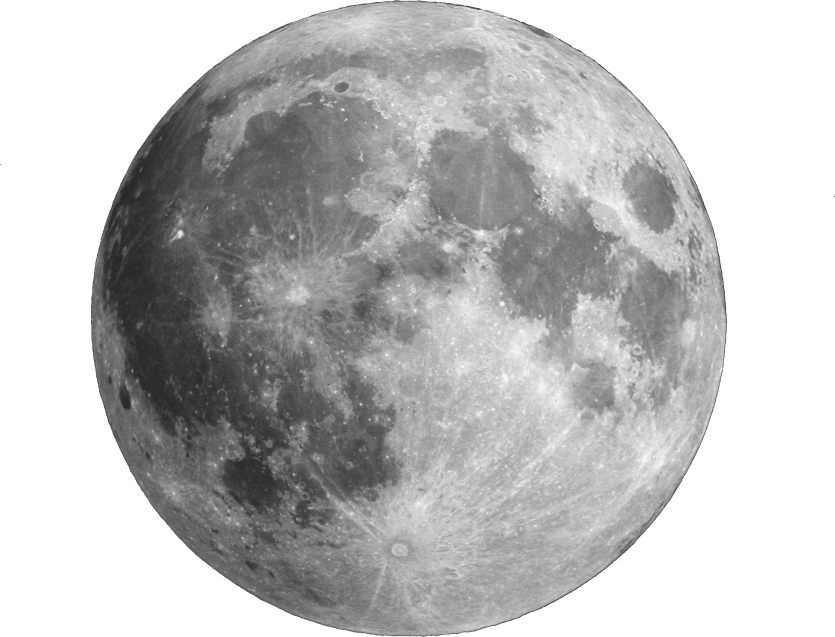
\includegraphics[width=0.9\textwidth]{assets/texture_samples/moon.png}\caption*{moon}\end{subfigure}
    \begin{subfigure}{0.18\textwidth}\centering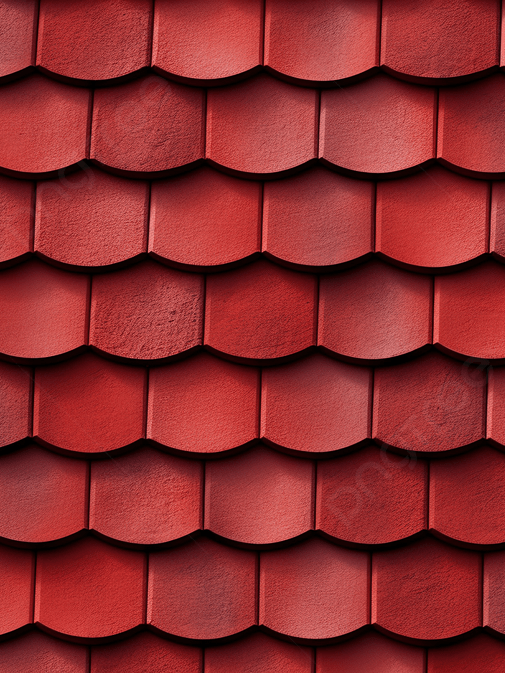
\includegraphics[width=0.9\textwidth]{assets/texture_samples/roof_tile.png}\caption*{roof\_tile}\end{subfigure}

    \vspace{0.3cm}

    \begin{subfigure}{0.18\textwidth}\centering
\includegraphics[width=0.9\textwidth]{assets/texture_samples/wood_plank.png}\caption*{wood\_plank}\end{subfigure}

    \caption{Texture sample sheet (all available samples).}
    \label{fig:texture-samples}
\end{figure}

\section{Day and Night Sky}
The sky rendering is driven by the day-night cycle and includes color interpolation, star visibility at night, and moon rendering in the celestial pass. The two captures below show the daytime and nighttime sky states used by the scene.

\begin{figure}[H]
    \centering
    \begin{subfigure}{0.48\textwidth}
        \centering
        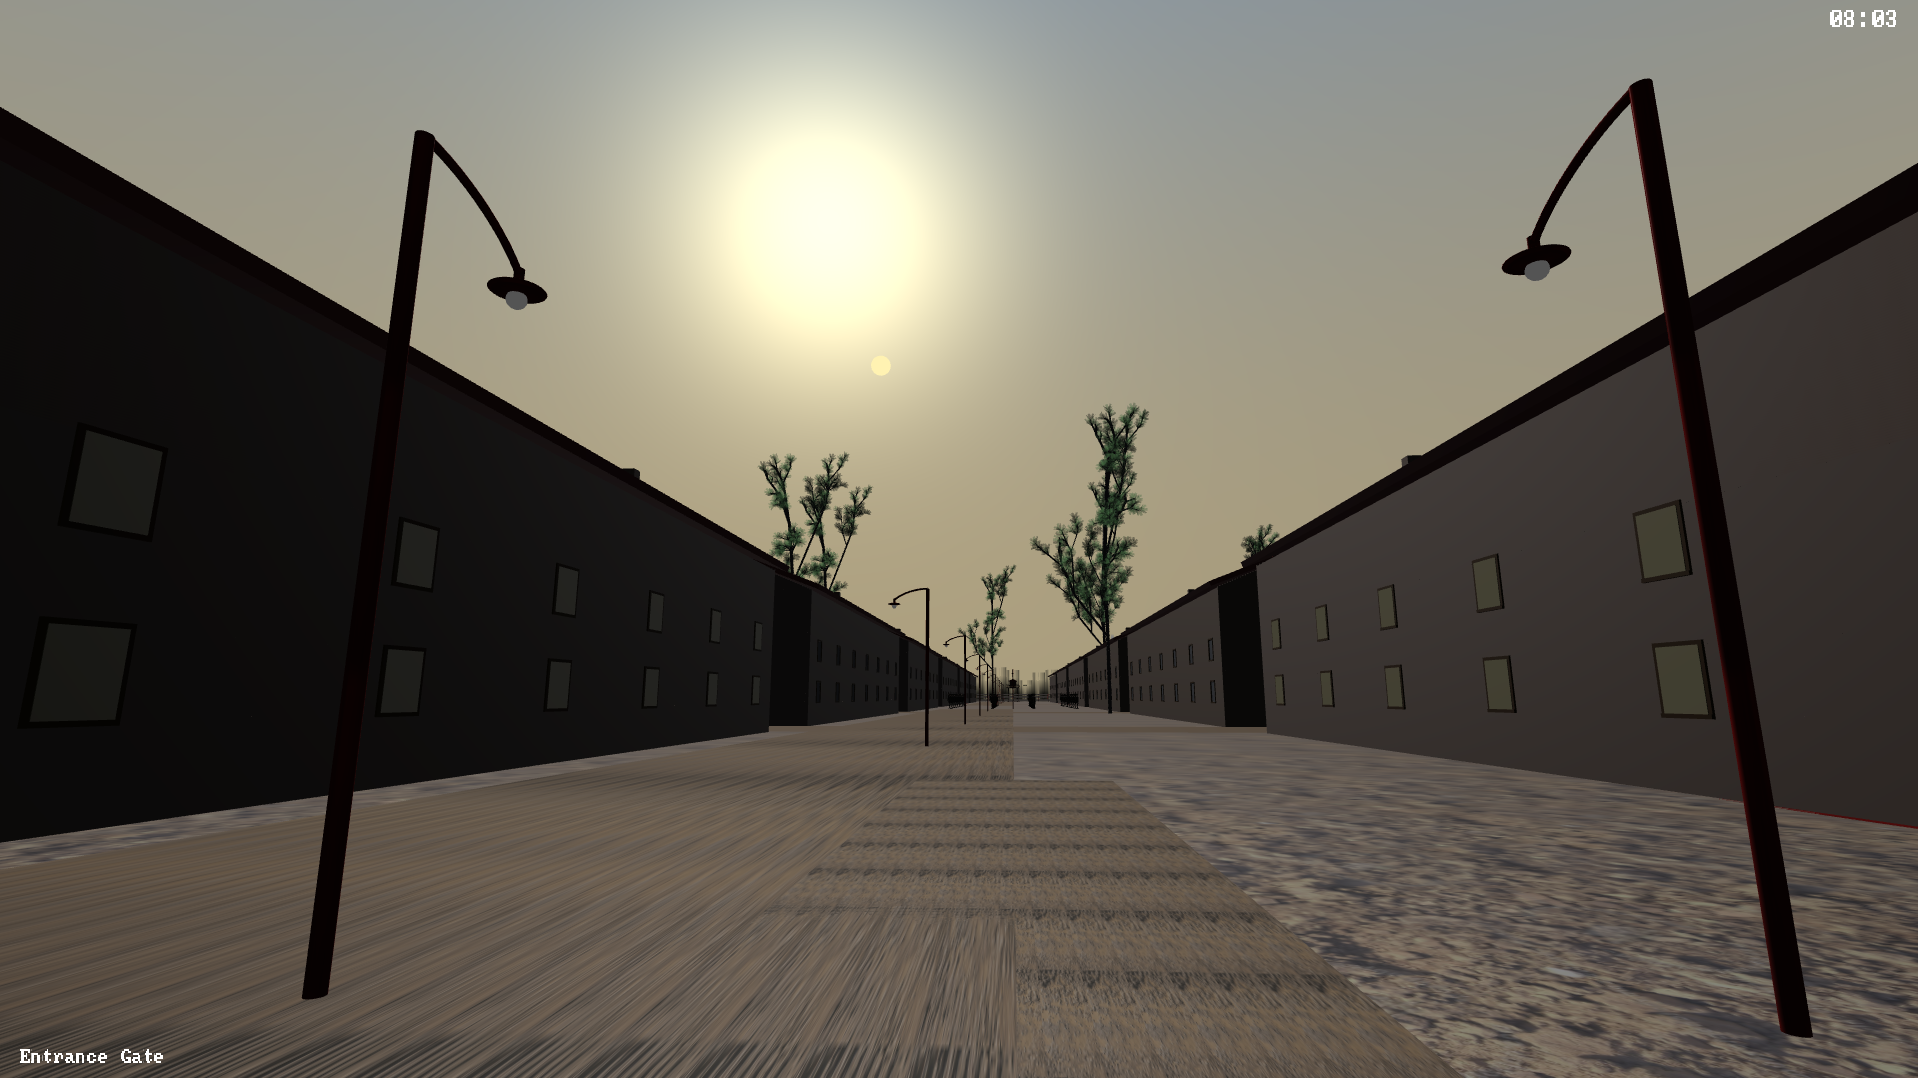
\includegraphics[width=\textwidth]{assets/screenshots/sky_day.png}
        \caption{Day sky state}
    \end{subfigure}
    \hfill
    \begin{subfigure}{0.48\textwidth}
        \centering
        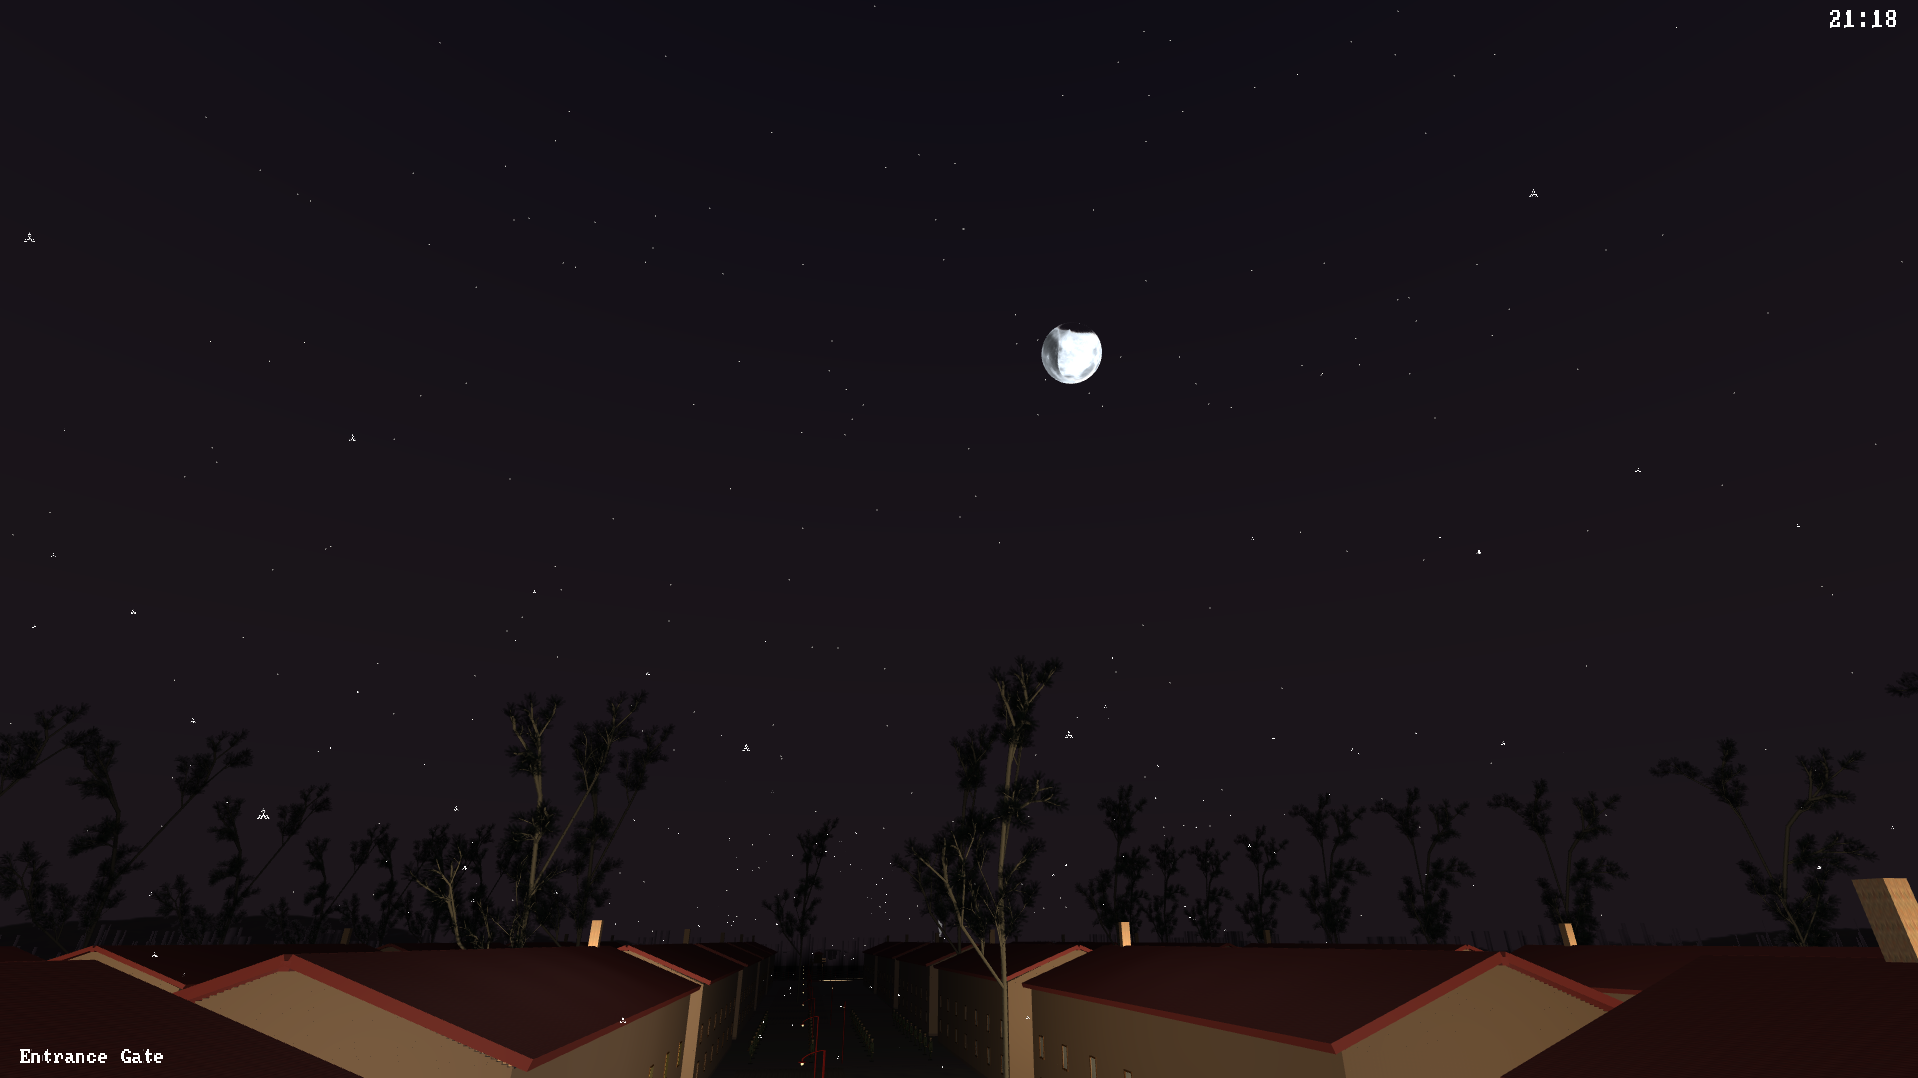
\includegraphics[width=\textwidth]{assets/screenshots/sky_night.png}
        \caption{Night sky state}
    \end{subfigure}
    \caption{Sky appearance across the day-night cycle.}
\end{figure}

\section{Scene Screenshots}
\begin{figure}[H]
    \centering
    \begin{subfigure}{0.48\textwidth}
        \centering
        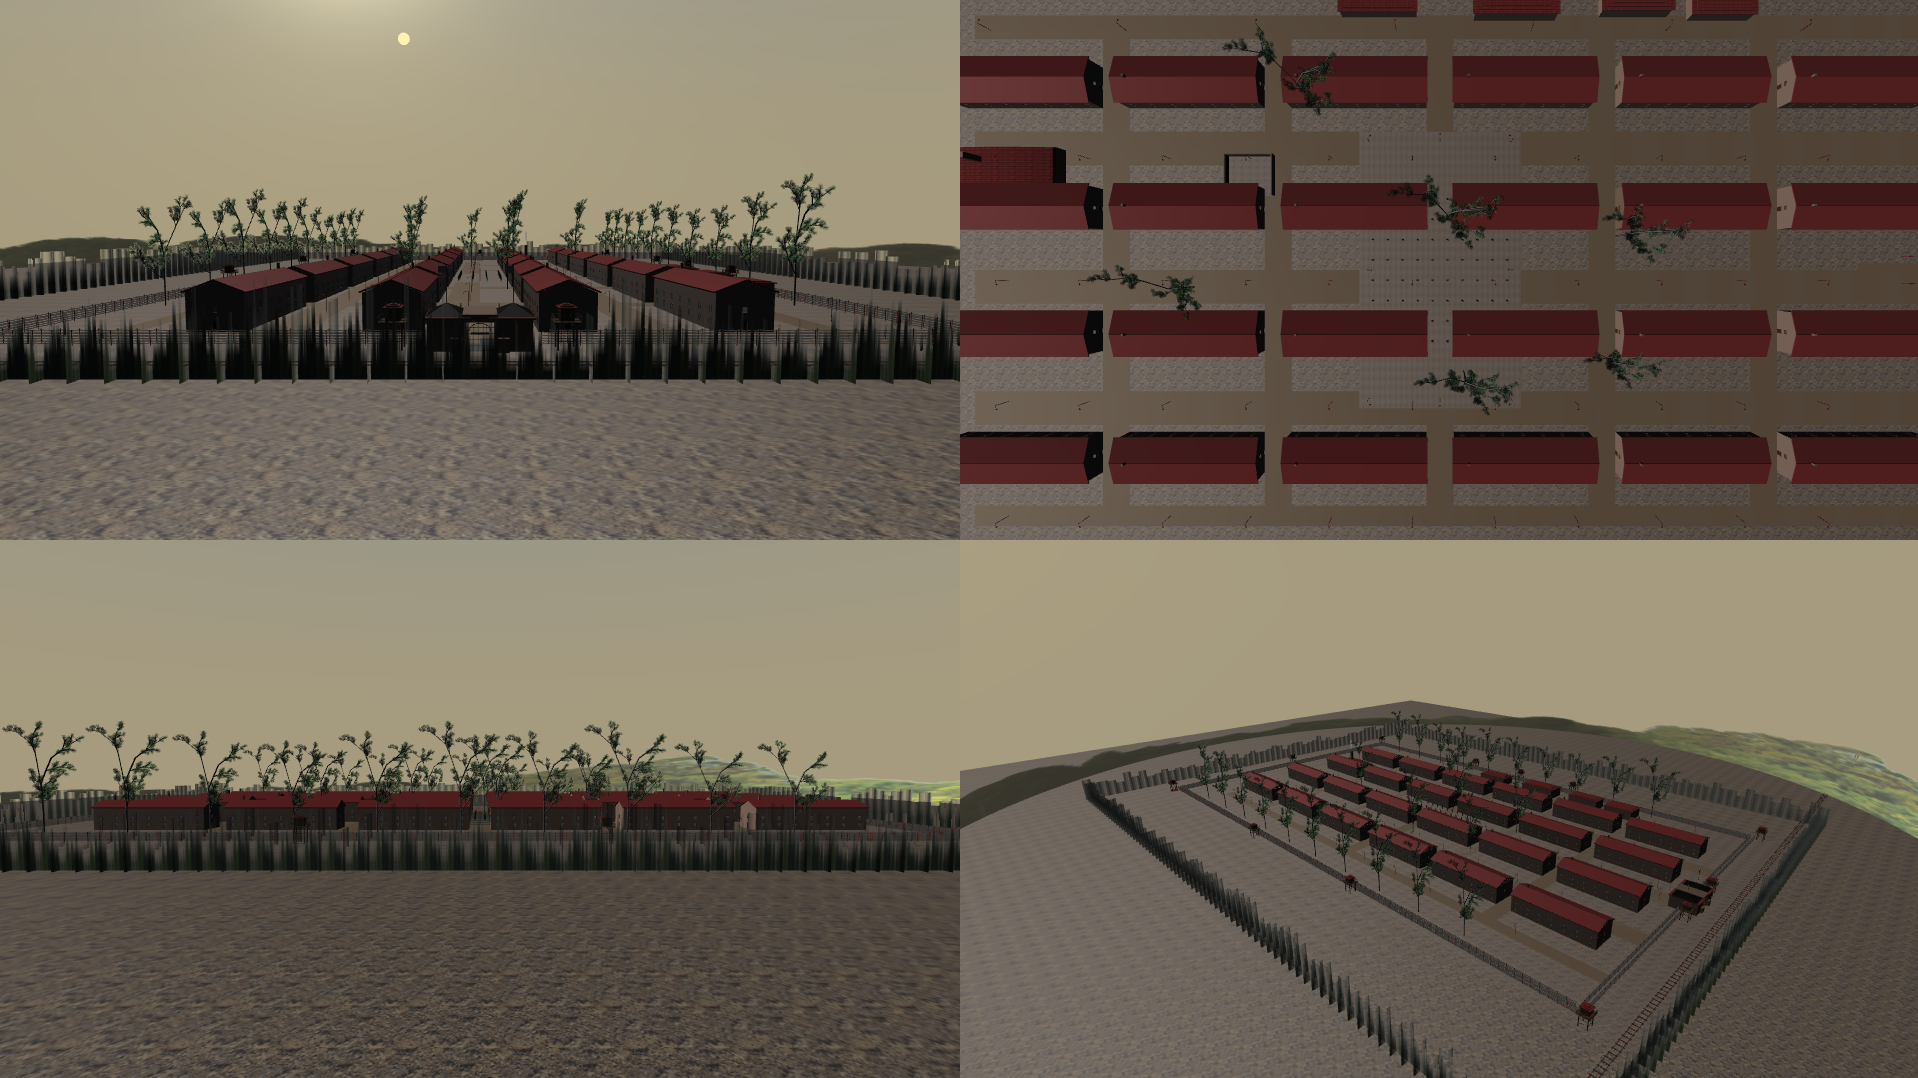
\includegraphics[width=\textwidth]{assets/screenshots/camp_day.png}
        \caption{Camp overview (day)}
    \end{subfigure}
    \hfill
    \begin{subfigure}{0.48\textwidth}
        \centering
        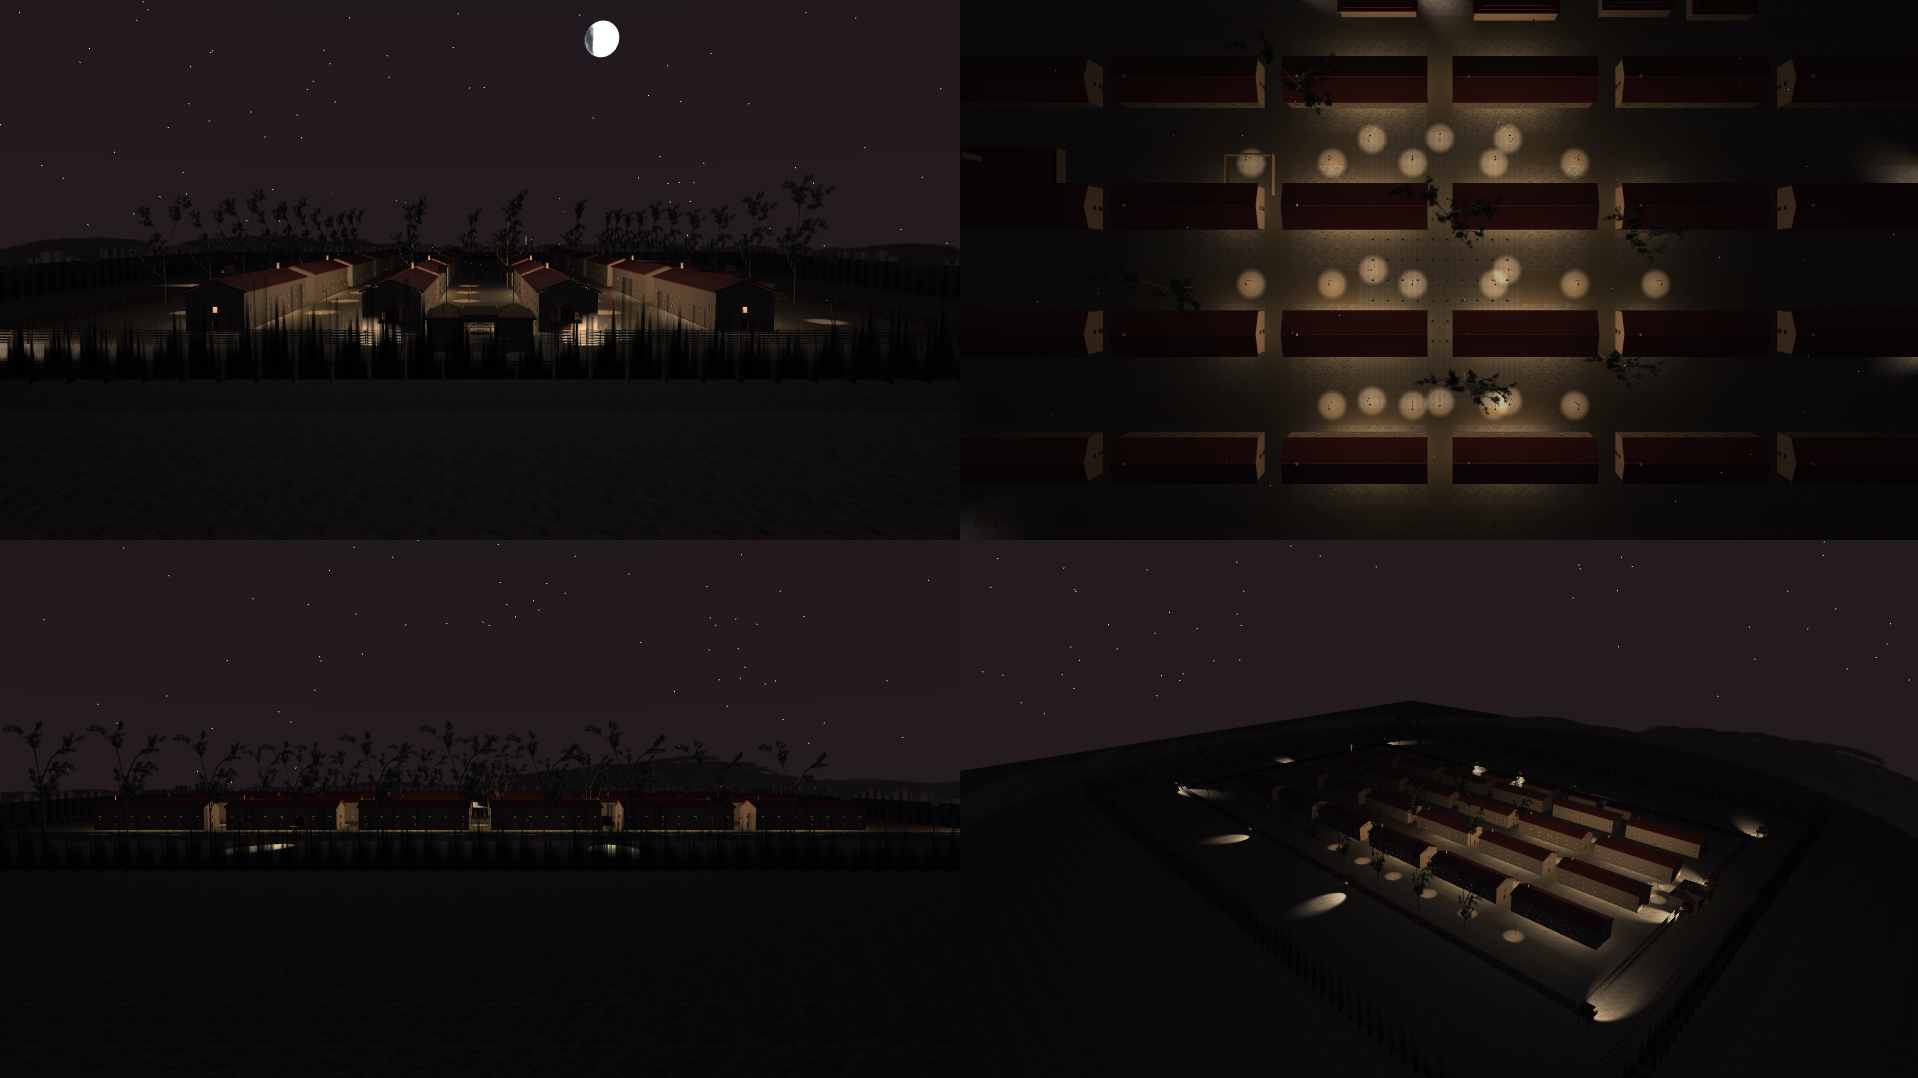
\includegraphics[width=\textwidth]{assets/screenshots/camp_night.png}
        \caption{Camp overview (night)}
    \end{subfigure}

    \vspace{0.3cm}

    \begin{subfigure}{0.48\textwidth}
        \centering
        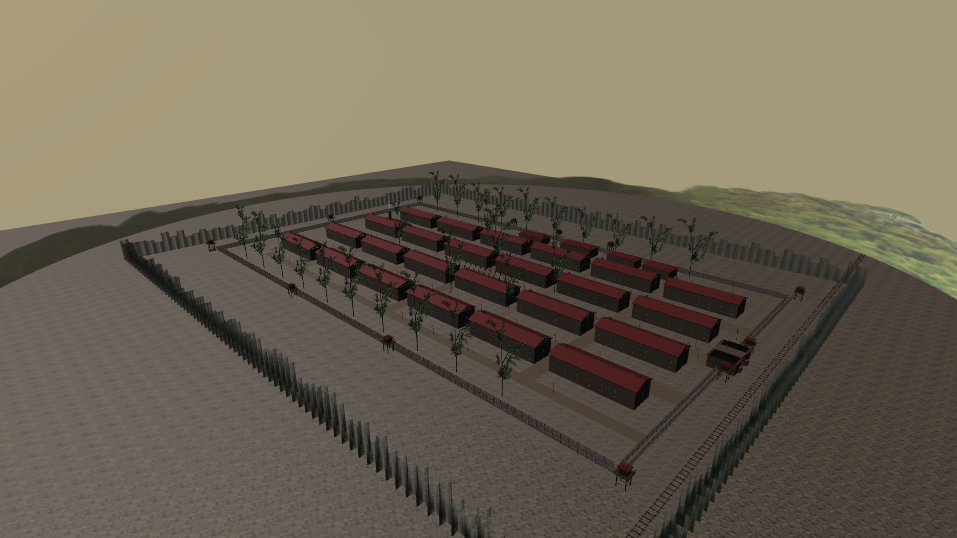
\includegraphics[width=\textwidth]{assets/screenshots/camp_isomeric.png}
        \caption{Bird's-eye/isometric view}
    \end{subfigure}
    \hfill
    \begin{subfigure}{0.48\textwidth}
        \centering
        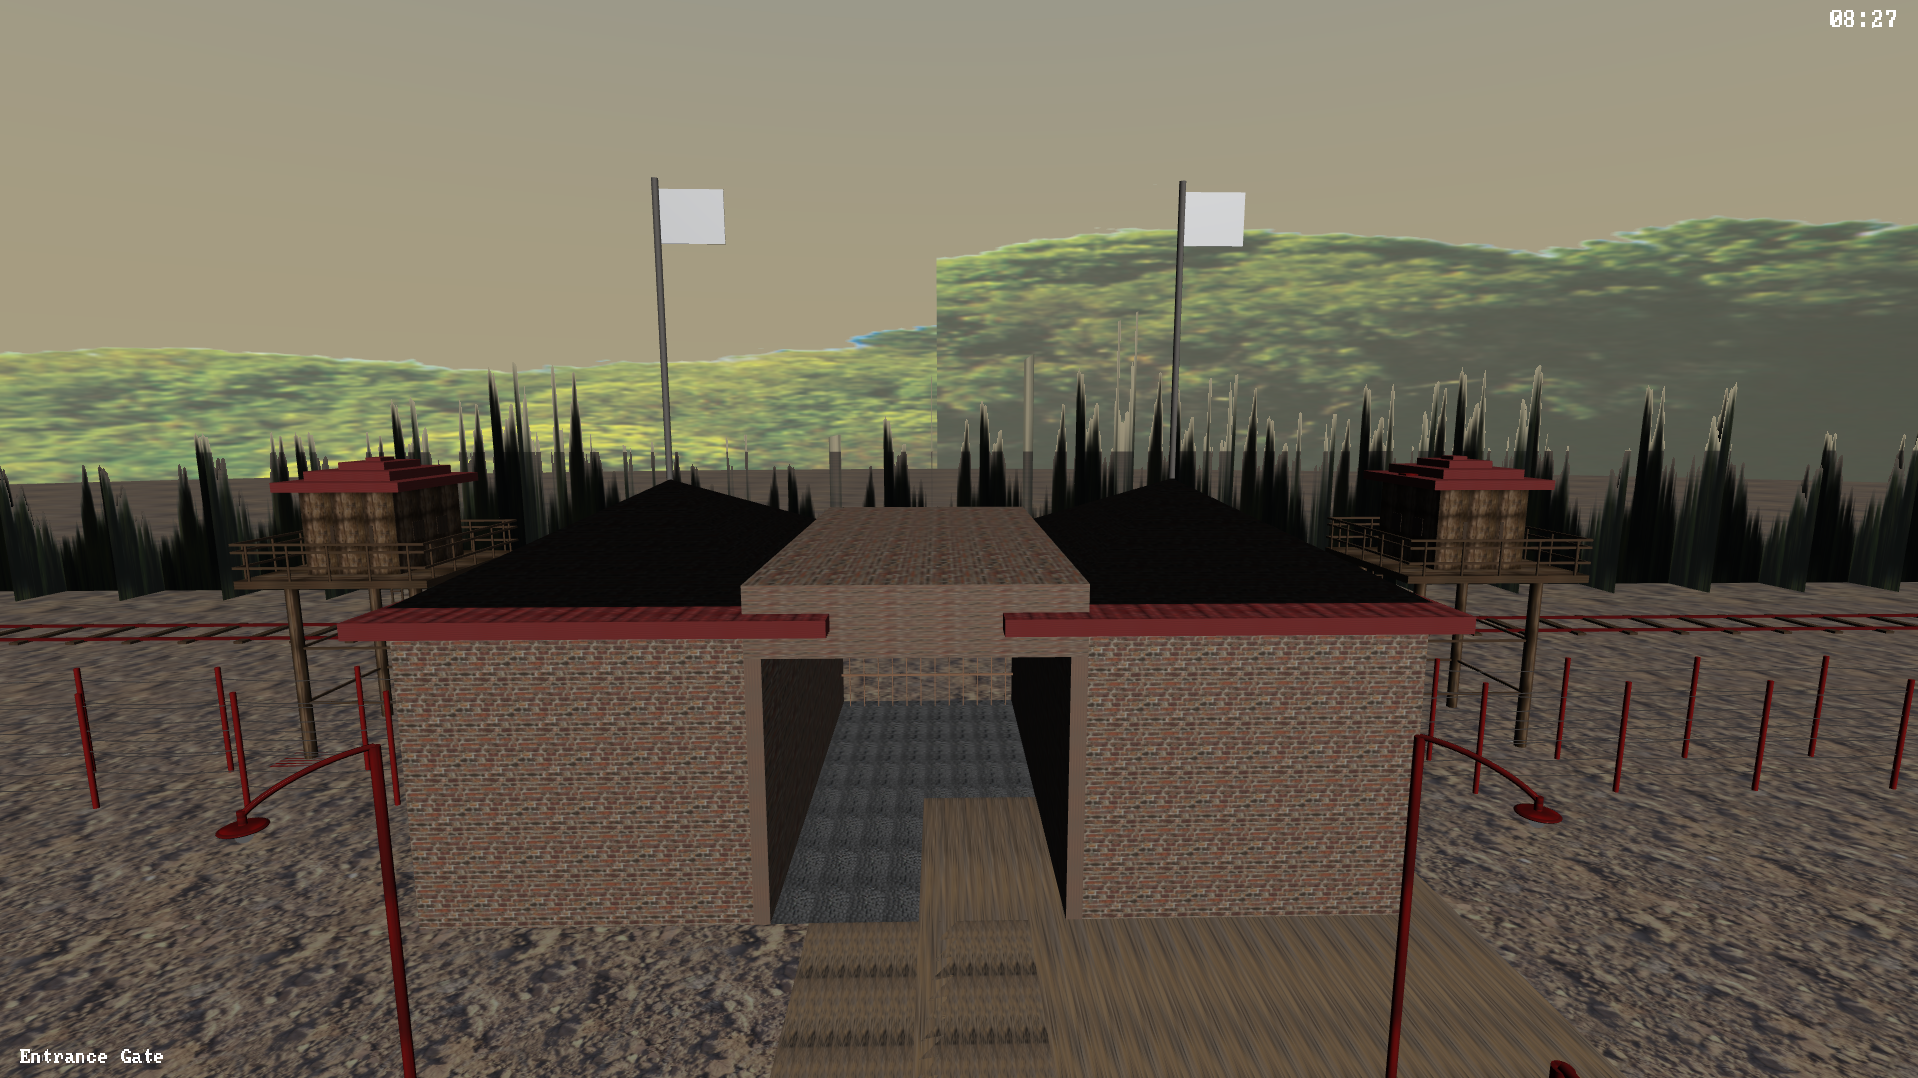
\includegraphics[width=\textwidth]{assets/screenshots/main_gate.png}
        \caption{Entrance gate area}
    \end{subfigure}
    \caption{Selected scene captures from implemented zones and view modes.}
\end{figure}

\begin{figure}[H]
    \centering
    \begin{subfigure}{0.48\textwidth}
        \centering
        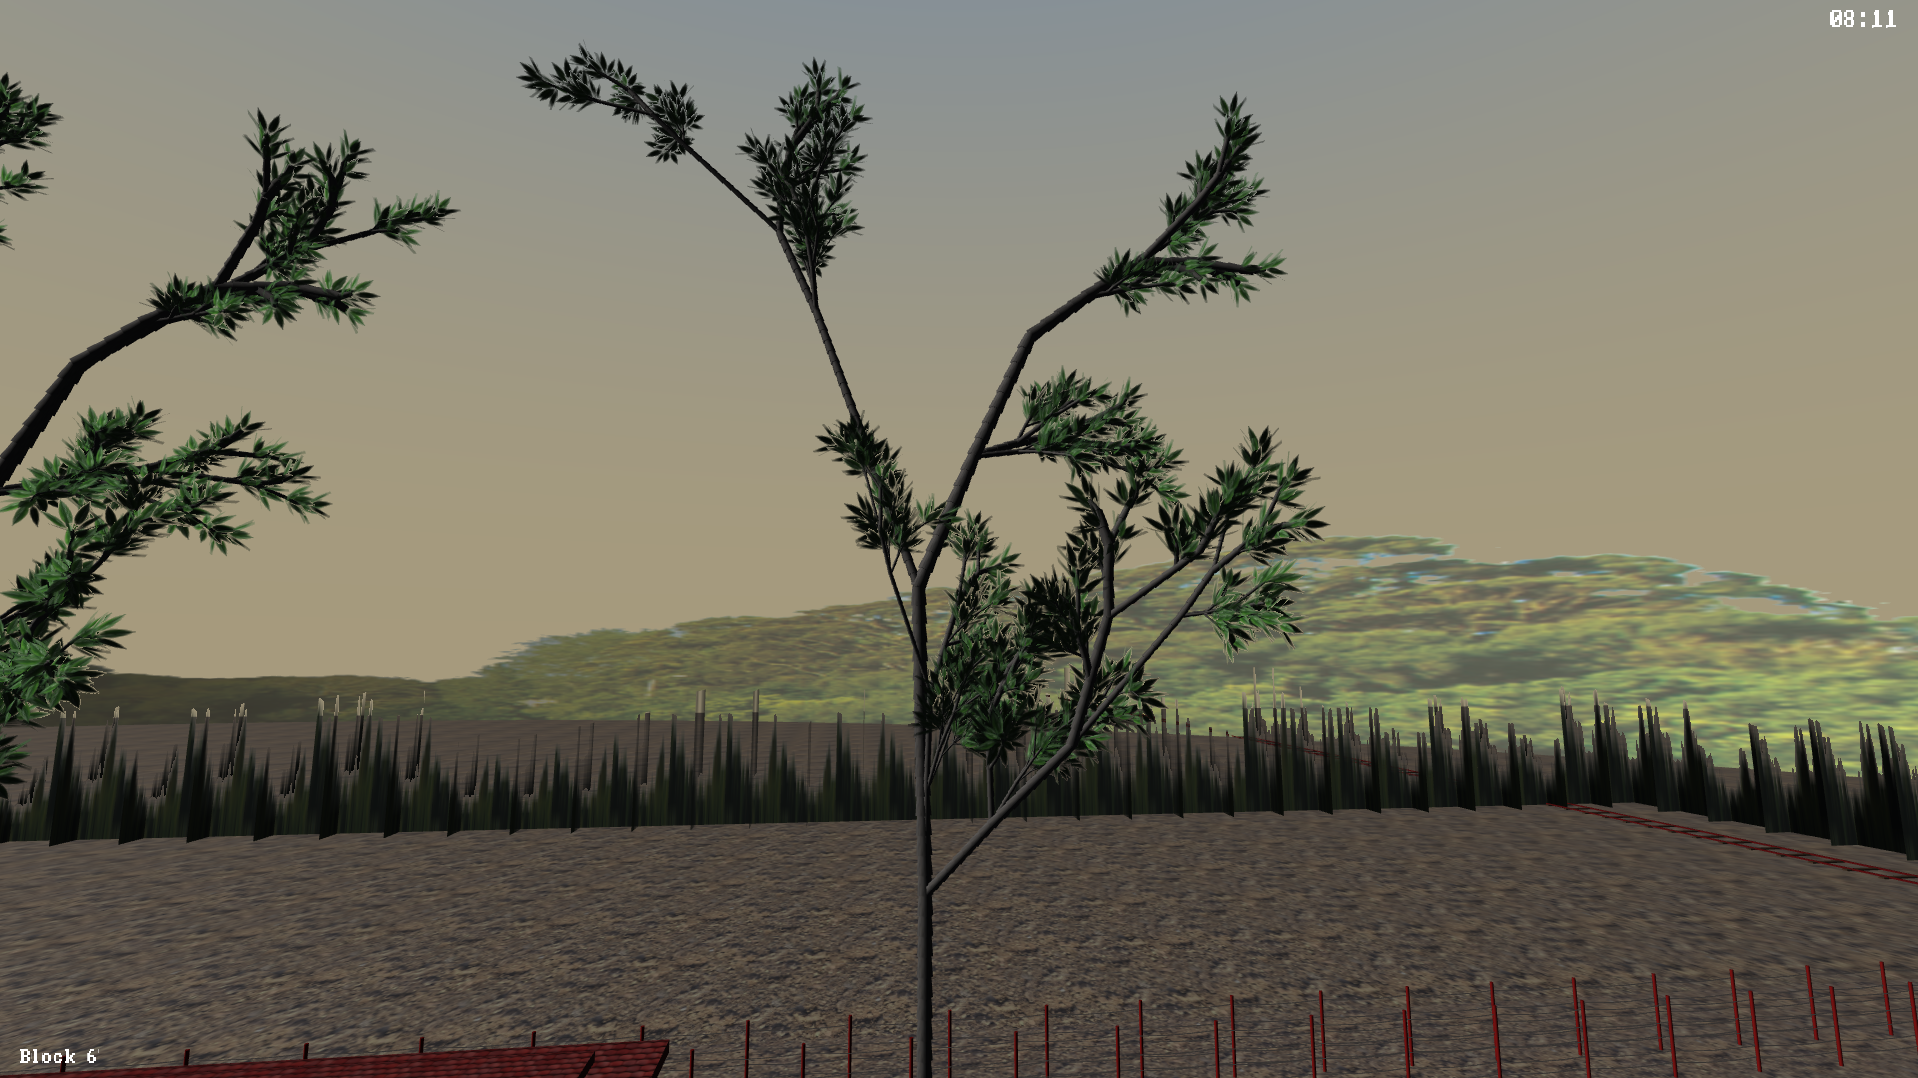
\includegraphics[width=\textwidth]{assets/screenshots/fractal_tree.png}
        \caption{Procedural L-system tree}
    \end{subfigure}
    \hfill
    \begin{subfigure}{0.48\textwidth}
        \centering
        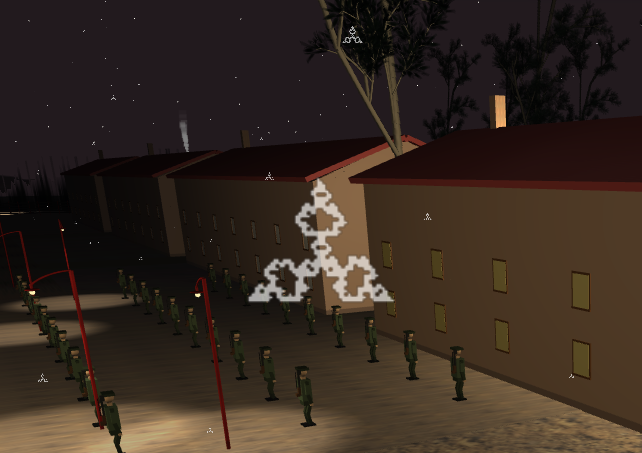
\includegraphics[width=\textwidth]{assets/screenshots/fractal_snowflake.png}
        \caption{Procedural snowflake overlay}
    \end{subfigure}
    \caption{Procedural and atmospheric features.}
\end{figure}

\section{Keyboard Controls}
\begin{table}[H]
\centering
\small
\caption{Keyboard controls in the current implementation}
\begin{tabular}{|p{0.15\textwidth}|p{0.75\textwidth}|}
\hline
\textbf{Key} & \textbf{Action} \\
\hline
\texttt{W A S D} & Move camera \\
\hline
\texttt{Shift} & Sprint \\
\hline
\texttt{Space / Left Ctrl} & Move camera up / down \\
\hline
\texttt{Mouse / Scroll} & Look / FOV zoom \\
\hline
\texttt{T} & Cycle time speed (pause/1x/8x/30x) \\
\hline
\texttt{H} & Toggle HUD \\
\hline
\texttt{C} & Toggle cursor lock \\
\hline
\texttt{F} & Toggle fullscreen \\
\hline
\texttt{G} & Toggle doors \\
\hline
\texttt{K} & Toggle windows \\
\hline
\texttt{J} & Trigger train run \\
\hline
\texttt{U / I} & Increase / decrease train speed \\
\hline
\texttt{P} & Toggle soldier parade \\
\hline
\texttt{V} & Toggle normal / 4-point view \\
\hline
\texttt{1 / 2 / 3 / 4} & Toggle ambient / diffuse / specular / emissive \\
\hline
\texttt{0} & Toggle all textures globally \\
\hline
\texttt{ESC} & Exit application \\
\hline
\end{tabular}
\end{table}

\section{Conclusion}
The implemented system is a complete, modular OpenGL reconstruction with stable multi-pass rendering, bounded dynamic lighting, procedural geometry, zone-level expansion, and runtime interaction controls. The interactive train and soldier courtyard modules along with interactive doors, windows and other controls integrate into the existing pipeline without changing the core scene architecture, demonstrating extensibility of the design.

\section{References}
\begin{enumerate}
    \item Khronos Group, \textit{OpenGL Reference Pages}. \url{https://registry.khronos.org/OpenGL-Refpages/}
    \item GLFW, \textit{GLFW 3 Documentation}. \url{https://www.glfw.org/documentation.html}
    \item G-Truc, \textit{GLM: OpenGL Mathematics}. \url{https://github.com/g-truc/glm}
    \item GLAD, \textit{OpenGL Loader Generator}. \url{https://glad.dav1d.de/}
\end{enumerate}

\end{document}
